\documentclass[a4paper,11pt]{article}
\pagestyle{headings}

\usepackage[utf8]{inputenc}
\usepackage{diagbox}
\usepackage[french]{babel}
\usepackage{graphicx}
\usepackage{float}
\usepackage{fullpage}
\usepackage{hyperref}
\usepackage{diagbox}
\usepackage{enumitem}
\usepackage[T1]{fontenc}
\usepackage[]{algorithm2e}
\graphicspath{{images/}}

\title{Reconnaissance de formes et apprentissage automatique Projet 2}
\author{Auriane Reverdell, Felix Hähnlein, Nicolas Violette, Romain Duléry}
\date{\today}

\setlength{\oddsidemargin}{0.2cm}
\setlength{\evensidemargin}{-0.7cm}
\setlength{\parindent}{30pt}
\setlength{\textwidth}{15cm}
\setlength{\textheight}{24cm}
\setlength{\topmargin}{-.5in}
\setlength{\parskip}{1ex}

\begin{document}

\maketitle
\vspace{1cm}

\section{Problématique et objectifs}

\section{Analyse quantitative}
    
    \subsection{Choix de l'évaluation}
        
        Pour évaluer l'algorithme, nous avons choisi d'utiliser des courbes Précision-Rappel. 
        Nous avons fait ce choix pour les raisons suivantes :\\\\
        Premièrement, l'implémentation d'{\it OpenCV} ne nous donne pas facilement accès au nombre de vrais négatifs, ce qui nous empêche de tracer des courbes ROC.
        Dans notre cas, les vrais négatifs sont les fenêtres et sous-fenêtres qui ont été rejetées par la cascade de features.
        Notre objectif dans ce TP étant d'examiner un détecteur de visages en tant que boîte noire, nous avons décidé de ne pas modifier le code source pour avoir accès au nombre de fenêtres rejetées.
        Néanmoins, nous avons essayé de récupérer ce nombre avec succès, mais nous nous sommes rendu compte qu'il était inexploitable, car il est beaucoup trop important.
        En effet, contrairement à la méthode étudiée pendant le premier TP où le nombre de ROI est maîtrisable, la détection de Viola-Jones utilise des ROI et des sous-fenêtres à plusieurs échelles ce qui rend $FP$ négligeable devant $TN$.
        Cela fait que le taux de faux positifs $FPR = \frac{FP}{FP+TN}$ sera toujours très proche de $0$.
        \\
        La construction des courbes Précision-Rappel nécessite la classification des détections obtenues par la fonction \verb!detectMultiScale! d'{\it OpenCV} et l'affection d'un score à chaque détection, qui nous permettra de décider pour une détection donnée si l'on accepte ou pas. La construction va être décrite plus en détail dans la section  \ref{construction_courbe}.
        
    \subsection{Classification des détections}
        
        La classification des détections joue un rôle important pour l'évaluation de l'algorithme.
        Il s'agit de décider si une détection est considérée comme un vrai positif, i.e. si nous pouvons considérer qu'elle a bien détecté un visage ou si il s'agit d'un faux positif, c'est-à-dire que l'algorithme a détecté une région comme étant un visage par erreur. Ces faux positifs peuvent par exemple être déclenchés par des régions qui ressemblent à un visage, comme c'est le cas pour la figure \ref{fig:mask_faux_positif}.
	    \begin{figure}[H]
	        \begin{center}
	    	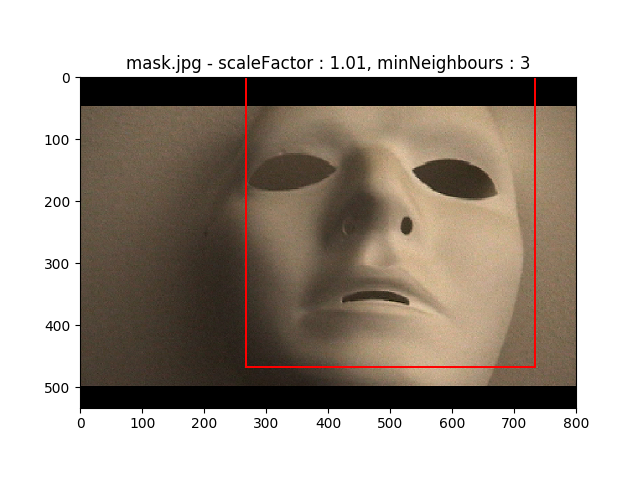
\includegraphics[scale = 0.6]{images/mask_1,01_3.png}
	    	\caption{Exemple de faux positifs}
	    	\label{fig:mask_faux_positif}
	        \end{center}
	    \end{figure}

        Pour décider s'il s'agit d'un vrai positif ou d'un faux positif, nous avons implémenté la méthode détaillée dans $[4]$.
        Il s'agit d'une méthode proposée par les créateurs de la base de données FDDB que nous utilisons dans le cadre de ce projet.
        \\
        La méthode consiste à trouver le couplage maximal dans un graphe biparti.
        Les sommets de ce graphe sont divisés en deux ensembles, l'ensemble des détections et l'ensemble des étiquettes, i.e. des vrais visages, annotés dans la base de données.
        Chaque détection partage une arête avec chaque étiquette, dont le poids est le rapport entre l'intersection et l'union des aires des deux régions.
        Ce poids correspond au taux de correspondance entre une détection et un vrai visage présent dans l'image.
        \\
        Nous calculons le couplage maximal grâce à la fonction \verb!scipy.optimize.linear_sum_assignment!, l'implémentation de l'algorithme hongrois.
        En sortie, nous nous intéressons à trois ensembles de sommets. 
        Les sommets qui comptent parmi les sommets de détections et qui font parti du couplage sont considérés comme des {\bf vrais posifits}.
        Ceux qui comptent parmi les sommets de détections et qui ne font pas parti du couplage sont considérés comme des {\bf faux posifits}.
        Les sommets qui sont des étiquettes et qui ne font pas parti du couplage sont considérés comme des {\bf faux négatifs}, il s'agit d'un visage qui n'a pas été détecté.
        \\
        \\
        Il est intéressant de noter que cette manière de classifier les détections implique qu'il ne peut y avoir qu'une seule détection par étiquette, même si le centre d'une deuxième détection est dans la région qui nous intéresse.
        Un exemple d'illustration se trouve dans la figure \ref{fig:false_positive_couplage}, où le faux positif est dessiné en jaune, les vrais positifs en bleu et les étiquettes en rouge.
	    \begin{figure}[H]
	        \begin{center}
	    	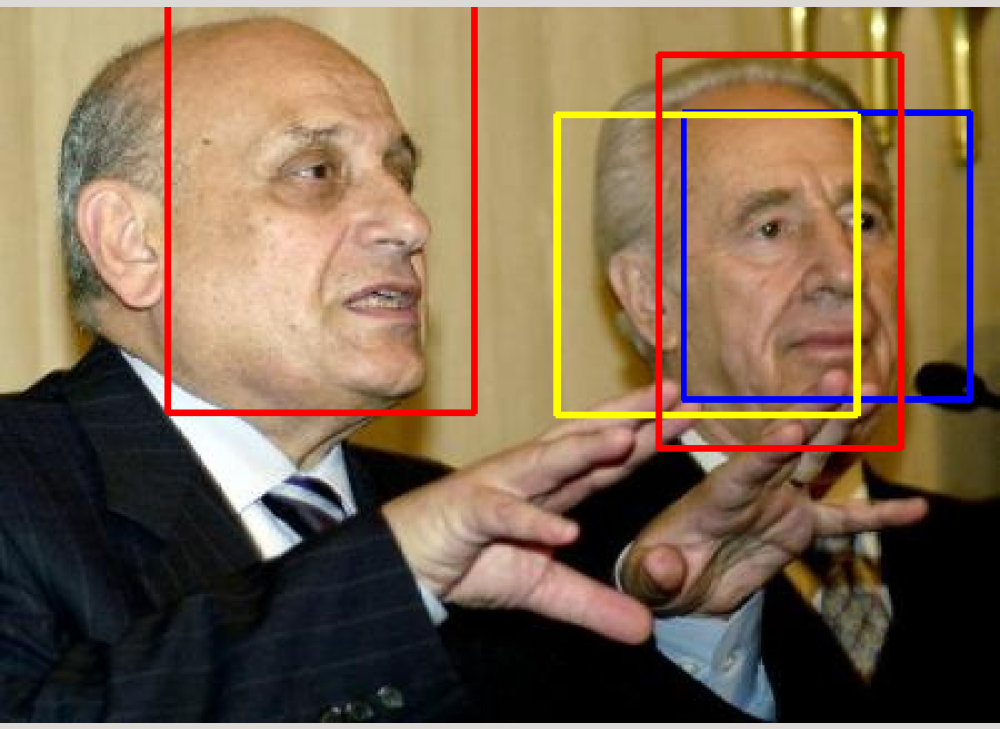
\includegraphics[scale = 0.4]{images/false_positive.png}
	    	\caption{Exemple de faux positifs à la sortie du couplage}
	    	\label{fig:false_positive_couplage}
	        \end{center}
	    \end{figure}

    \subsection{Affectation des détections par un score}

        Pour la construction de la courbe Précision-Rappel, nous avons besoin de faire varier un seuil d'acceptance de détections.
        La comparaison d'une détection avec ce seuil nécessite l'accès à un score qui traduit la confiance que nous avons en cette détection.
        {\it OpenCV} nous donne accès à un tel score via la fonction \verb!detectMultiScale3! qui ne nous renvoie pas seulement l'ensemble des détections mais aussi pour chaque détection le dernier niveau qu'elle a parcouru et la somme qu'elle a accumulé en ce niveau. 
        \\
        Rappelons qu'une éventuelle détection parcourt tous les niveaux d'une cascade de classification, dont chacun est composé de plusieurs features.
        Chacune de ces features va contribuer à un score de confiance du niveau en question. 
        Si le score dépasse un certain seuil, alors on passe au niveau suivant, sinon on rejette l'imagette.
        \\
        Nous obtenons donc en sortie de la fonction \verb!detectMultiScale3! le score de confiance du dernier niveau de la cascade.

    \subsection{Construction de la courbe Précision-Rappel}
    \label{construction_courbe}
        
        Après avoir obtenu les scores de confiance et après avoir classifié les détections, nous passons à la construction de la courbe Précision-Rappel.
        Pour cela, nous parcourons les détections en ordre croissant de scores de confiance.
        Au début, $TP$, $FP$ et $FN$ valent respectivement le nombre total de vrais positifs, faux positifs et faux négatifs, présents dans l'ensemble des images parcourues.
        Ensuite, à chaque étape du parcours des scores, nous procédons de la manière suivante.

        \begin{algorithm}[H]
        \eIf{détection courante est un TP}{
            TP = TP-1\;
            FN = FN+1\;
        }{
            FP = FP-1\;
        }
        \end{algorithm}
        Autrement dit, nous rejetons progressivement les détections en faisant augmenter notre seuil d'acceptance et dans le cas d'un vrai positif, nous augmentons le nombre de faux négatifs, car nous détectons un visage en moins.
        \\
        Enfin, nous faisons remarquer que nos courbes ne vont pas jusqu'à la limite théorique, qui est le point $(1,0)$. 
        Ce point correspond au cas où il n'y a plus de faux négatif, i.e. le système de détection nous renvoie toutes les détections possibles.
        Ce cas n'arrivera jamais avec l'impléménetation donnée, on aura donc toujours un nombre de faux négatifs minimum.
        Cela correspond visuellement au moment où nos courbes s'arrêtent brusquement (voir la section \ref{results}).

    \subsection{Analyse des résultats}
        
        Un exemple de courbe obtenue se trouve sur la figure \ref{fig:minN_1}.
        Pour la construire, nous avons parcouru le premier dossier de la base de données FDDB pour différents facteurs d'échelle et un nombre de voisins minimum fixé.
        En plus de cela, afin de les comparer, nous avons calculé l'aire sous la courbe (AUC) pour chacune des courbes.
        
    \label{results}
	\begin{figure}[H]
	    \begin{center}
		\includegraphics[scale = 0.4]{images/courbes/folder_01_minN_1.png}
		\caption{courbe Précision-Rappel: minNeighbours: 1, dossier: 1}
		\label{fig:minN_1}
	    \end{center}
	\end{figure}
        Nous constatons plusieurs choses.
        \\
        Premièrement, nous remarquons que l'AUC est nettement meilleure pour des facteurs d'échelle entre $1.05$ et $1.35$ que pour le reste des valeurs.
        En effet, en prenant un facteur d'échelle trop grand, la pyramide d'images construite par l'algorithme risque d'être trop grossière pour capter tous les visages.
        Visuellement, nous pouvons constater cela à deux endroits. 
        D'une part, la courbe s'arrête plus tôt en abscisse parce que nous retirons moins d'informations pertinentes des images, i.e. $FN$ augmente.
        Et d'autre part, la courbe baisse en ordonnée parce que la détection devient moins précise, i.e. $TP$ diminue.

    \subsection{Analyse des paramètres}
        
        Afin de construire un système de détection de visage automatisé, nous devons déterminer les paramètres qui donnent les meilleurs résultats dans la plupart des cas.
        En l'occurence, nous avons deux paramètres à régler, qui sont le {\bf scaleFactor} et {\bf minNeighbours}.
        Avant de présenter nos résultats, voici quelques remarques.
        \begin{itemize}
            \item scaleFactor
                En théorie, ce paramètre détermine le nombre de niveau intermédiaire de la pyramide d'images utilisée par l'algorithme pour être invariant à l'échelle.
                En réalité, ce n'est pas l'image qui va être agrandit ou rétrécit plusieurs fois, mais le filtre.
                Un scaleFactor de $1.1$ signifie que la taille du filtre va être multiplié par $1.1$ jusqu'à ce que sa taille dépasse les dimensions de l'image.
                Contrairement à d'autres caractéristiques appliquables sous forme de filtre, comme par exemple le filtre gaussien, les features utilisés ici ont l'avantage qu'en combinaison avec des images intégrales, nous pouvons les calculer en $\mathcal{O}(1)$ peu importe la taille du feature.
                \\
                Ceci implique que le temps d'exécution est linéaire en fonction du scaleFactor.
                Alors notre système va encore être utilisable, même si nous choisissons d'augmenter la précision du filtre.
            \item minNeighbours
                Après avoir déterminé tous les rectangles contenant éventuellement des visages, l'implémentation d'{\it OpenCV} les regroupe.
                Ce regroupement se fait via la fonction \verb!groupRectangles! qui rejete tout rectangle n'ayant pas au moins minNeighbours rectangles voisins.
                \\
                Le choix de ce paramètre n'a pas de conséquence directe sur la performance de l'algorithme, mais il présente un seuil d'acceptance.
                Il s'agit d'un post-traitement, appliqué aux détections à la sortie de la cascade.
        \end{itemize}

        Nous avons parcourus des scaleFactor de $1.05$ à $1.95$ avec un pas de $0.05$ et des minNeighbours de $1$ à $10$.
        Dans le tableau \ref{tab:parmeters}, nous avons listé les AUCs obtenues, les courbes correspondantes se trouvent en Annexe A \ref{annexes_a}.

        \begin{table}
            \centering
            \resizebox{\textwidth}{!}{\begin{tabular}{|l|*{10}r|}
                \hline
                \diagbox{scaleFactor}{minNeighbours} &1&2&3&4&5&6&7&8&9&10\\
                \hline
                1.05 &  0.84029 & 0.84735  & {\bf 0.85245} & {\bf 0.85088}  & {\bf 0.85269}  & {\bf 0.85011}  & 0.84939 & 0.84883  & 0.84708 & 0.84949 \\
                1.1  &  0.83821 & 0.84674  & 0.84748 & 0.84371  & 0.84082  & 0.84016  & 0.84002 & 0.83755  & 0.82833 & 0.82778 \\
                1.15 &  0.84274 & 0.84632  & 0.84196 & 0.83934  & 0.83488  & 0.8329   & 0.82738 & 0.82063  & 0.81625 & 0.81087 \\
                1.2  &  0.84598 & 0.83982  & 0.8376  & 0.83104  & 0.83084  & 0.82644  & 0.81963 & 0.81282  & 0.80319 & 0.7934 \\
                1.25 &  0.83938 & 0.83657  & 0.82415 & 0.82326  & 0.8154   & 0.80982  & 0.7953  & 0.78433  & 0.77056 & 0.76311 \\
                1.3  &  0.83718 & 0.82962  & 0.82697 & 0.81574  & 0.80791  & 0.79536  & 0.78226 & 0.76851  & 0.75292 & 0.74078 \\
                1.35 &  0.82528 & 0.81632  & 0.80712 & 0.79981  & 0.78691  & 0.77415  & 0.76117 & 0.75146  & 0.73981 & 0.72524 \\
                1.4  &  0.69126 & 0.68491  & 0.67319 & 0.66591  & 0.66005  & 0.65284  & 0.65533 & 0.64393  & 0.63196 & 0.6033  \\
                1.45 &  0.7122  & 0.71735  & 0.72019 & 0.72076  & 0.70242  & 0.69236  & 0.67942 & 0.66287  & 0.64525 & 0.63706 \\
                1.5  &  0.72374 & 0.72254  & 0.71336 & 0.70939  & 0.70495  & 0.69852  & 0.68064 & 0.6618   & 0.6431  & 0.6266 \\
                1.55 &  0.73429 & 0.72779  & 0.71558 & 0.70943  & 0.70448  & 0.68986  & 0.67078 & 0.65628  & 0.64569 & 0.62822 \\
                1.6  &  0.75299 & 0.74188  & 0.74484 & 0.72646  & 0.71067  & 0.69824  & 0.68601 & 0.65673  & 0.63463 & 0.60931 \\
                1.65 &  0.74678 & 0.73193  & 0.72451 & 0.7098   & 0.6984   & 0.68226  & 0.67318 & 0.66668  & 0.64784 & 0.63301 \\
                1.7  &  0.74519 & 0.73482  & 0.72441 & 0.71607  & 0.71669  & 0.70112  & 0.68877 & 0.67005  & 0.64676 & 0.62197 \\
                1.75 &  0.77955 & 0.76254  & 0.74319 & 0.72626  & 0.70672  & 0.68429  & 0.66372 & 0.65628  & 0.63925 & 0.61608 \\
                1.8  &  0.76135 & 0.74061  & 0.72924 & 0.70982  & 0.70426  & 0.68071  & 0.66716 & 0.65049  & 0.6301  & 0.61359 \\
                1.85 &  0.75225 & 0.73927  & 0.72222 & 0.70164  & 0.68589  & 0.67757  & 0.65767 & 0.63962  & 0.63107 & 0.61165 \\
                1.9  &  0.75961 & 0.74894  & 0.72936 & 0.71159  & 0.69853  & 0.67885  & 0.65829 & 0.63756  & 0.62039 & 0.60874 \\
                1.95 &  0.75568 & 0.73907  & 0.71448 & 0.70373  & 0.68064  & 0.6699   & 0.65728 & 0.63689  & 0.61748 & 0.6 \\
                \hline
            \end{tabular}}
            \caption{AUCs obtenues pour le dossier 1}
            \label{tab:parmeters}
        \end{table}

        Nous constatons que les valeurs maximales se trouvent au bord de notre plage de valeurs de test. 
        Nous avons donc testé des scaleFactor encore plus petits pour optimiser l'AUC.
        


%TODO : faire une vraie analyse sur les paramètres
%TODO : invariances, robustesse au bruit, à la compression
\section{Analyse qualitative des détections}
    
    \subsection{Orientation du visage}
	
	Dans l'image suivante (figure \ref{fig:visage_or1}), l'orientation du visage varie
	progressivement, cela nous montre exactement l'orientation à partir de laquelle la
	reconnaissance ne marche plus. Nous remarquons ici que la détection dépend de la présence
	des deux yeux, dès que l'un d'eux n'est plus visible ou occulté, la détection ne fonctionne
	plus.

	\begin{figure}[H]
	    \begin{center}
		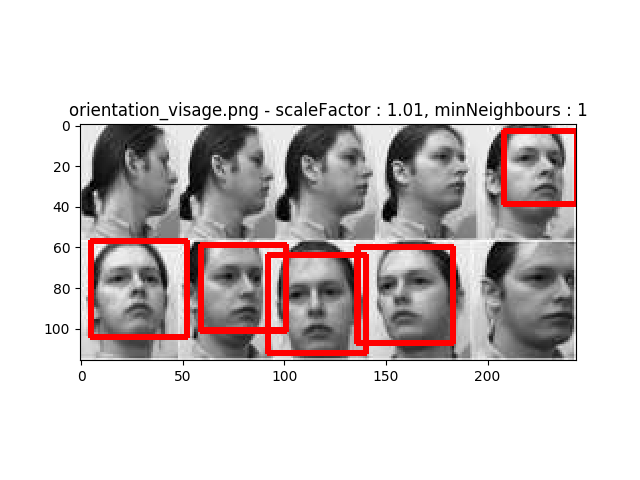
\includegraphics[scale = 0.6]{images/orientation_visage_1,01_1.png}
		\caption{Variation de l'orientation du visage - min neighbours = 1}
		\label{fig:visage_or1}
	    \end{center}
	\end{figure}

	Si l'on augmente \textit{minNeighbours}, rien ne change jusqu'à 3 (figure
	\ref{fig:visage_or2}) puis le nombre de TP diminue. En effet, cette variable
	(en l'augmentant) sert à limiter le nombre de FP. Or, comme il n'y a pas
	d'environnement d'arrière plan propices aux fausses détections, les fausses détections sont
	inexistantes, même avec un \textit{minNeighbours} à 1. Le \textit{scaleFactor} (à 1\%)
	permet,	quant à	lui, des détections précises (on ne saute pas trop rapidement à une petite 
	échelle).

	\begin{figure}[H]
	    \begin{center}
		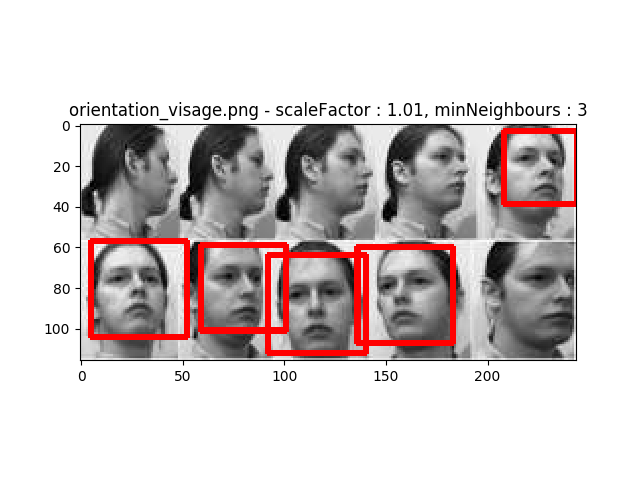
\includegraphics[scale = 0.6]{images/orientation_visage_1,01_3.png}
		\caption{Variation de l'orientation du visage - min neighbours = 3}
		\label{fig:visage_or2}
	    \end{center}
	\end{figure}

    \subsection{Expressions du visage}
	
	On pourrait se demander ce que deviennent les détections sur un visage avec des expressions
	différentes voire même avec les yeux fermés. On remarque sur la figure \ref{fig:visage_exp}
	que le détecteur est robuste à ces changements.

	\begin{figure}[H]
	    \begin{center}
		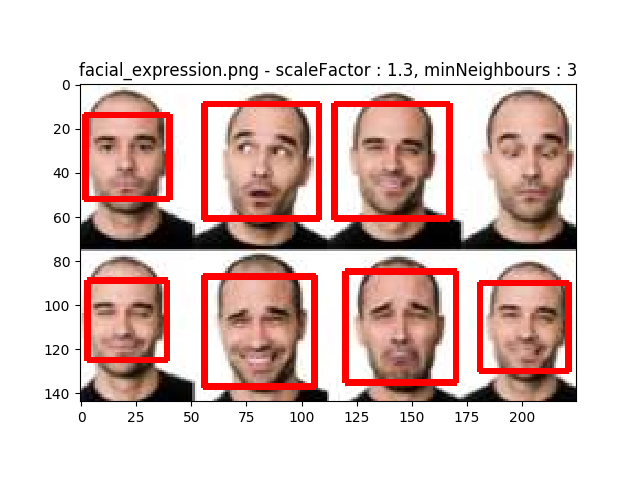
\includegraphics[scale = 0.6]{images/facial_expression_1,3_3.png}
		\caption{Changement d'expressions du visage}
		\label{fig:visage_exp}
	    \end{center}
	\end{figure}

    
    \subsection{Singes}

	Le singe est détecté lorsque le	\textit{scaleFactor} et le \textit{minNeighbours} sont
	relativement bas (figure \ref{fig:singe}), dès que l'on augmente à 1.06 le
	\textit{scaleFactor} la reconnaissance ne se fait plus correctement.
	En effet on peut supposer que les features sont moins
	adaptés aux variations de gris des visages des singes, i.e., même en mettant le
	\textit{minNeighbours} à 0 nous avons relativement peu de détections sur le vrai visage.

	\begin{figure}[H]
	    \begin{center}
		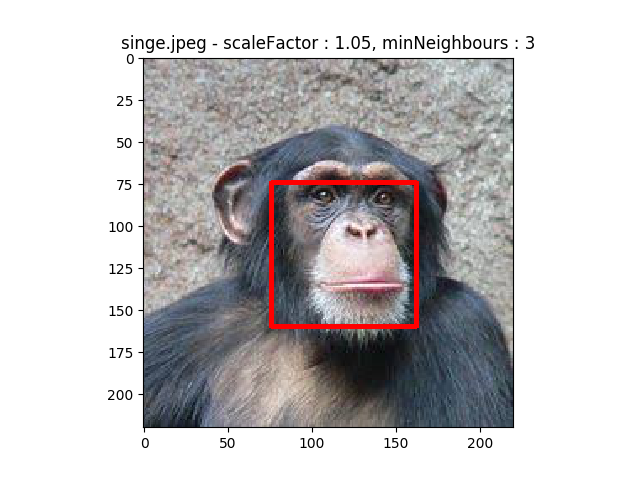
\includegraphics[scale = 0.6]{images/singe_1,05_3.png}
		\caption{Reconnaissance d'un singe}
		\label{fig:singe}
	    \end{center}
	\end{figure}

	Si l'on prend des paramètres identiques pour la reconnaissance du gorille (cela nous semble
	faisable car il y a une importante zone d'ombre au niveau des yeux du gorille), la
	reconnaissance ne marche pas, il faut augmenter le \textit{scaleFactor} à 1.02 pour qu'on
	ait une détection (cf figure \ref{fig:singe2}).

	\begin{figure}[H]
	    \begin{center}
		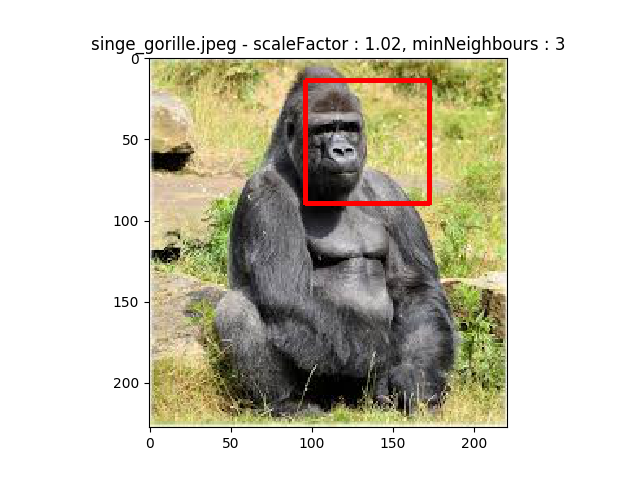
\includegraphics[scale = 0.6]{images/singe_gorille_1,02_3.png}
		\caption{Reconnaissance d'un gorille - scaleFactor = 1.02}
		\label{fig:singe2}
	    \end{center}
	\end{figure}

    \subsection{Occultations}
	
	Comme on l'a vu précédemment, lorsque qu'un oeil disparaît, la détection de visage ne se
	fait plus, on peut donc se demander ce qui se passe dans le cas d'une occultation de la
	bouche ou encore dans le cas d'un déguisement de pirate.

	\subsubsection{Oeil de pirate}

	    Ce que l'on voit ici (figure \ref{fig:pirate}), c'est que, même si l'oeil est occulté, tant
	    que la partie des yeux est foncée, le visage est bien détecté alors que lorsque l'on
	    compare avec l'occultation du visage par les mains (figure \ref{fig:mains}), il n'y a
	    plus de différentiel d'intensité (qui est ce sur quoi est basé l'algorithme de
	    Viola-Jones), les TP sont donc inexistants (même avec les paramètres au plus bas).

	    \begin{figure}[H]
	        \begin{center}
		   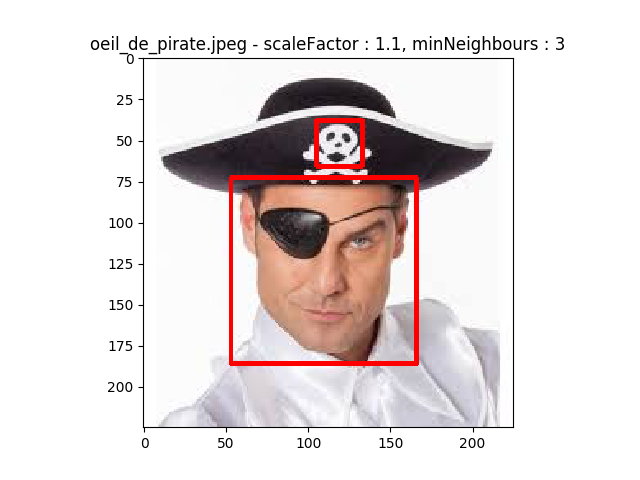
\includegraphics[scale = 0.6]{images/oeil_de_pirate_1,1_3.png}
		   \caption{Reconnaissance d'un visage occulté}
		   \label{fig:pirate}
	        \end{center}
	    \end{figure}

	    \begin{figure}[H]
	        \begin{center}
		   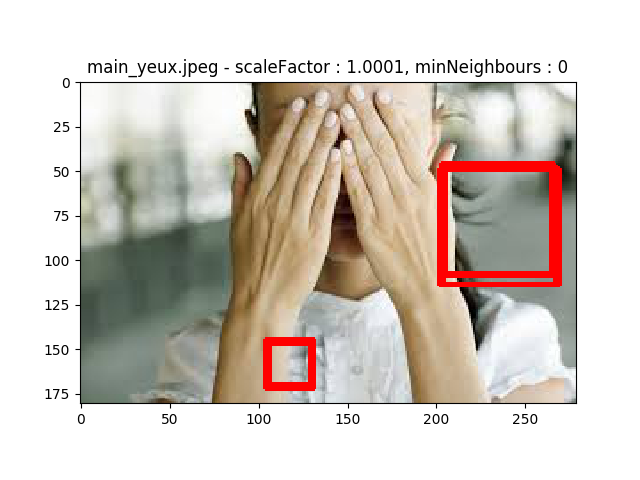
\includegraphics[scale = 0.6]{images/main_yeux_1,0001_0.png}
		   \caption{Reconnaissance d'un visage occulté par les mains}
		   \label{fig:mains}
	        \end{center}
	    \end{figure}

	\subsubsection{Lunettes de soleil}

	    Ces lunettes de soleil étant noires (figure \ref{fig:lunette}), la détection fonctionne très bien : il y a un gros
	    différentiel d'intensité entre les lunettes et le reste du visage.

	    \begin{figure}[H]
	        \begin{center}
		   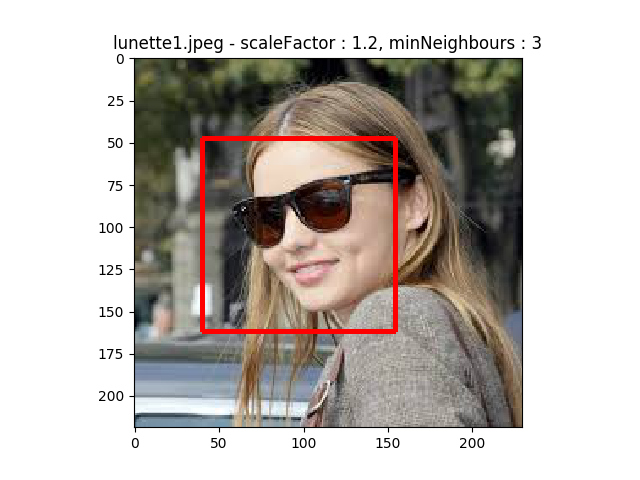
\includegraphics[scale = 0.6]{images/lunette1_1,2_3.png}
		   \caption{Reconnaissance d'un visage occulté par des lunettes de soleil}
		   \label{fig:lunette}
	        \end{center}
	    \end{figure}
	
	\subsubsection{Illumination}

	    Comme nous l'avons précisé, ci-dessus, la méthode de Viola-Jones est basée sur les
	    intensités. L'illumination est donc l'un des critères qui peut fortement affecter les
	    détections. En effet, un visage partiellement ombragé donnera du fil à retordre à
	    l'algorithme. \\

	    Lorsque l'on regarde la figure \ref{fig:illumination}, nous remarquons que les visages
	    non détectés sont ceux qui ne laissent pas transparaître un \textit{feature} évident. Au
	    contraire, si l'on prend le visage en haut à droite, nous pouvons prédire qu'il
	    conviendra parfaitement à un \textit{feature} binaire.


	    \begin{figure}[H]
	        \begin{center}
		   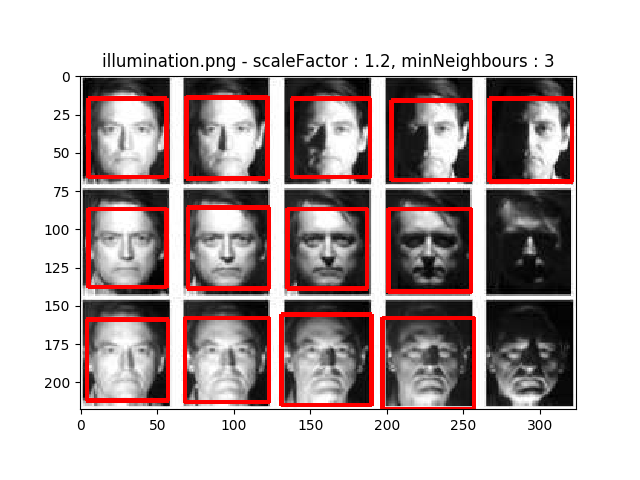
\includegraphics[scale = 0.6]{images/illumination_1,2_3.png}
		   \caption{Reconnaissance d'un visage ombragé}
		   \label{fig:illumination}
	        \end{center}
	    \end{figure}
	

\section{Illustrations en utilisant la webcam}

\section{Bibliographie}
\flushleft
$[1]$ - \url{http://www.ijcttjournal.org/2015/Volume25/number-1/IJCTT-V25P110.pdf} \\
$[2]$ - \url{http://www-prima.inrialpes.fr/Prima/jlc/Courses/2017/PRML/Viola-Jones-CVPR2001.pdf} \\
$[3]$ - \url{http://www.ipol.im/pub/art/2014/104/article.pdf} \\
$[4]$ - \url{http://vis-www.cs.umass.edu/fddb/fddb.pdf}

\section{Annexes}
    
    \subsection{Annexes: A}
    \label{annexes_a}

%    \label{results}
%	\begin{figure}[H]
%	    \begin{center}
%		\includegraphics[scale = 0.4]{images/courbes/folder_01_minN_2.png}
%		\caption{courbe Précision-Rappel: minNeighbours: 2, dossier: 1}
%		\label{fig:minN_2}
%	    \end{center}
%	\end{figure}
%
%    \label{results}
%	\begin{figure}[H]
%	    \begin{center}
%		\includegraphics[scale = 0.4]{images/courbes/folder_01_minN_3.png}
%		\caption{courbe Précision-Rappel: minNeighbours: 3, dossier: 1}
%		\label{fig:minN_2}
%	    \end{center}
%	\end{figure}
%
%    \label{results}
%	\begin{figure}[H]
%	    \begin{center}
%		\includegraphics[scale = 0.4]{images/courbes/folder_01_minN_4.png}
%		\caption{courbe Précision-Rappel: minNeighbours: 4, dossier: 1}
%		\label{fig:minN_2}
%	    \end{center}
%	\end{figure}
%
%    \label{results}
%	\begin{figure}[H]
%	    \begin{center}
%		\includegraphics[scale = 0.4]{images/courbes/folder_01_minN_5.png}
%		\caption{courbe Précision-Rappel: minNeighbours: 5, dossier: 1}
%		\label{fig:minN_2}
%	    \end{center}
%	\end{figure}
%
%    \label{results}
%	\begin{figure}[H]
%	    \begin{center}
%		\includegraphics[scale = 0.4]{images/courbes/folder_01_minN_6.png}
%		\caption{courbe Précision-Rappel: minNeighbours: 6, dossier: 1}
%		\label{fig:minN_2}
%	    \end{center}
%	\end{figure}
%
%    \label{results}
%	\begin{figure}[H]
%	    \begin{center}
%		\includegraphics[scale = 0.4]{images/courbes/folder_01_minN_7.png}
%		\caption{courbe Précision-Rappel: minNeighbours: 7, dossier: 1}
%		\label{fig:minN_2}
%	    \end{center}
%	\end{figure}
%
%    \label{results}
%	\begin{figure}[H]
%	    \begin{center}
%		\includegraphics[scale = 0.4]{images/courbes/folder_01_minN_8.png}
%		\caption{courbe Précision-Rappel: minNeighbours: 8, dossier: 1}
%		\label{fig:minN_2}
%	    \end{center}
%	\end{figure}
%
%    \label{results}
%	\begin{figure}[H]
%	    \begin{center}
%		\includegraphics[scale = 0.4]{images/courbes/folder_01_minN_9.png}
%		\caption{courbe Précision-Rappel: minNeighbours: 9, dossier: 1}
%		\label{fig:minN_2}
%	    \end{center}
%	\end{figure}
%
%    \label{results}
%	\begin{figure}[H]
%	    \begin{center}
%		\includegraphics[scale = 0.4]{images/courbes/folder_01_minN_10.png}
%		\caption{courbe Précision-Rappel: minNeighbours: 10, dossier: 1}
%		\label{fig:minN_2}
%	    \end{center}
%	\end{figure}


\end{document}
